
\chapter{Data Aggregation}
First step towards this project is to fetch our data from Twitter. The data is classified into two
groups, relevant and irrelevant. We will be spending most of our time with the relevant data.


\section{Data Classification}
\label{sec:data_classification}
To carry out our experiments, we will need to filter out irrelevant tweets. Irrelevant tweets are
tweets which we do not really care about. Some examples include:

\begin{itemize}
  \item \textit{Every day I'm levelling! And now I'm level 19 in \#CSRClassics for iPhone!}
  \item \textit{Yes, our apple juice and cider are both GMO-free.}
  \item \textit{I just had my first carmel apple}
\end{itemize}

All three tweets could be regarded as relevant but for our use case, they are not. This is because
we are only interested in tweets that contain personal opinions about Apple Incorporated. Examples
of relevant tweets include: their thoughts
\begin{itemize}
  \item \textit{Once you get hooked to \#Mac, you will definitely go back to \#Windows! Lol!}
  \item \textit{If Tim Cook at Apple knows anything about him, it'd be to stay away from Icahn.}
\end{itemize}

Of course we can manually classify this data but when we have millions of tweets, this becomes
impracticable. This is where we employ some classification algorithms to assist us. This is a
three step process and we will discuss them in the next sub sections.

\subsection{Preparing train data}
\begin{figure}
  \begin{center}
    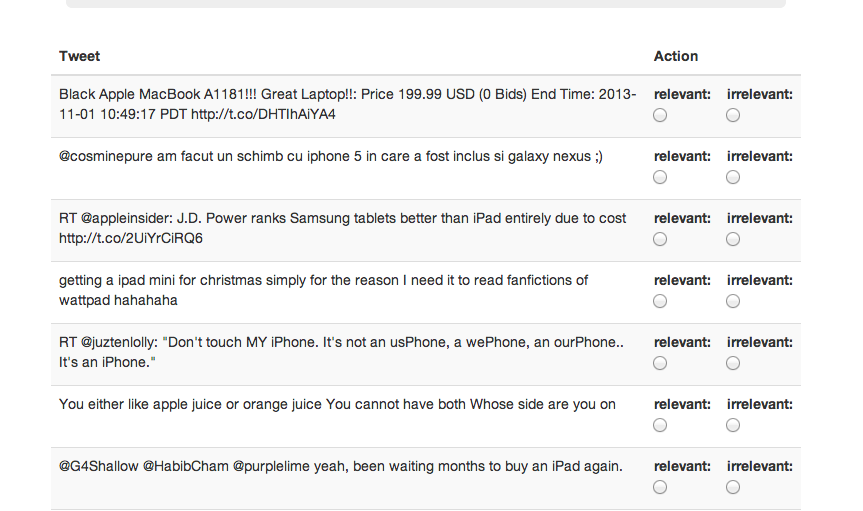
\includegraphics[scale=0.6]{figures/datalabeller}
  \end{center}
  \caption{The data labelling application}
\label{fig:labeller}
\end{figure}

Train data, also known as a training set is a set of data used to train a knowledge database, in
this case, a classifier. Our training set will be created by manually labelling a fraction of our
dataset. People write in different ways on Twitter and trying to create a new training set to
encompass all possibilities would be very time consuming and intractable. To make this process a
little easier, a web application for labelling tweets was created. Figure~\ref{fig:labeller} is a
screen shot of what the application looks like.

\begin{figure}
  \begin{center}
    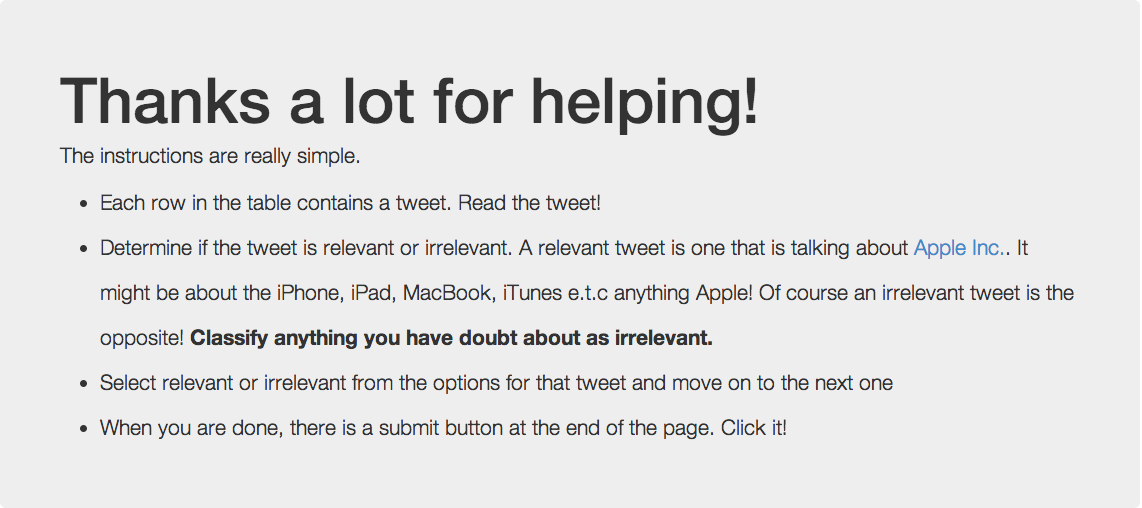
\includegraphics[scale=0.4]{figures/labeller_instructions}
  \end{center}
  \caption{Instructions on how to label the tweets}
\label{fig:labeller_instructions}
\end{figure}

While using the web application in Figure~\ref{fig:labeller} makes labelling tweets easier and a
little quicker, it does not change the fact the we still have to manually label a plethora of
tweets. To speed up this process even further, the data labeller was made public and the labelling
was crowd sourced. A list of instructions (Figure~\ref{fig:labeller_instructions}) were also given
to anyone who helped label the tweets.

One problem with crowd sourcing this task is that people have different opinions about what is
relevant and what is not. In an attempt to solve this problem, each tweet was classified twice. A
tweet classified as relevant gets a score of 1 and an irrelevant tweet gets 0. This means that if a
tweet was classified twice as relevant, it should have a score of 2 and a tweet classified as
irrelevant twice should have a score of 0. Tweets that have been classified twice and have a total
score of 1 are tweets that have been classified as both relevant and irrelevant. These are tweets
that we have to classify ourselves into a group. While this is not an assured way of getting the
best training set, it gives us a certain level of confidence about our training set. It is also
arguably much better than single handedly creating the training set.

\subsection{Training a classifier}
As discussed in Section~\ref{sec:bg_naive_bayes}, a Na\"{i}ve Bayes Classifier is a probabilistic
classifier which is based on the Bayes Theorem. We will train one and use it to classify the tweets
into relevant and irrelevant groups.

Unfortunately, the classifier takes as input a vector space representation of our tweets and not the
actual text. This means we have to convert our tweets into a vector representation of some sort. We
will be using the \textbf{bag of words model} in this study but before we transform the tweets, we
have to pre-process the tweets.

\subsubsection{Preprocessing}
\label{sec:preprocessing}
Preprocessing are the tasks we have to carry out before the main transformation of the tweets to a
vector space model. Firstly, we'll peruse through our tweets to remove new line characters and
links and stop words. We then take each tweet and convert it into a list of \textit{n-grams}.

Some tweets have special characters like new lines, excess spaces and Unicode characters. These
characters are noisy features we have to remove them, we make use of a regular expression. Every
programming language has a function to strip a text off newlines and whitespace and it can be
easily done in one line of code. Removing the links from the text is a little more complex and the
``easiest'' way to do this would be to use a regular expression. \cite{friedl2006mastering} in his
book \textit{Mastering Regular Expressions} describes regular expressions as a very flexible mini
language that is used for text processing. The regular expression we will be using to find links in
our text is
\begin{verbatim}
  {(https?:\/\/)?([\da-z\.-]+)\.([a-z\.]{2,6})([\/\w \.-]*)*\/?}
\end{verbatim}

Unfortunately, all a regular expression can do is search for patterns in text. Luckily, most
programming languages provides support regular expressions so all we have to do is search for the
pattern in each tweet and use the language features to replace the matched pattern with nothing(an
empty string preferably).

The next step is to remove stop words in each tweet. \cite{wilbur1992automatic} defines a stop word
as ``\textit{a word which may be identified as a word that has the same likelihood of occurring in
those documents not relevant to a query as in those documents relevant to the query.}'' In layman's
terms, stop words are words that occur in every document irrespective of the document's relevance.
Stop words are usually the most common word in a language, English in this case. Some examples include
\textit{and}, \textit{or}, \textit{the} etc. Removal of stop words from text usually results in
better model performance.
%TODO: reference a table in a future section that proves this.

% Finally, we convert each tweet to a list of \textit{n-grams}


% \subsubsection{Converting tweets to bag-of-words representation}
% The bag of words model is a common representation of text that involves

% In other to analyse how well our classifier works, we will measure the classifier's accuracy,
% precision and recall. We will also look into why we need all three evaluation techniques.

